\documentclass[conference]{IEEEtran}
\IEEEoverridecommandlockouts
% The preceding line is only needed to identify funding in the first footnote. If that is unneeded, please comment it out.
\usepackage{cite}
\usepackage{amsmath,amssymb,amsfonts}
\usepackage{algorithmic}
\usepackage{graphicx}
\usepackage{listings}
\usepackage{multirow}
\newcommand\YAMLcolonstyle{\color{red}\mdseries}
\newcommand\YAMLkeystyle{\color{black}\bfseries}
\newcommand\YAMLvaluestyle{\color{blue}\mdseries}

\makeatletter

% here is a macro expanding to the name of the language
% (handy if you decide to change it further down the road)
\newcommand\language@yaml{yaml}

\expandafter\expandafter\expandafter\lstdefinelanguage
\expandafter{\language@yaml}
{
  keywords={true,false,null,y,n},
  keywordstyle=\color{darkgray}\bfseries,
  basicstyle=\YAMLkeystyle,                                 % assuming a key comes first
  sensitive=false,
  comment=[l]{\#},
  morecomment=[s]{/*}{*/},
  commentstyle=\color{purple}\ttfamily,
  stringstyle=\YAMLvaluestyle\ttfamily,
  moredelim=[l][\color{orange}]{\&},
  moredelim=[l][\color{magenta}]{*},
  moredelim=**[il][\YAMLcolonstyle{:}\YAMLvaluestyle]{:},   % switch to value style at :
  morestring=[b]',
  morestring=[b]",
  literate =    {---}{{\ProcessThreeDashes}}3
                {>}{{\textcolor{red}\textgreater}}1     
                {|}{{\textcolor{red}\textbar}}1 
                {\ -\ }{{\mdseries\ -\ }}3,
}

% switch to key style at EOL
\lst@AddToHook{EveryLine}{\ifx\lst@language\language@yaml\YAMLkeystyle\fi}
\makeatother

\newcommand\ProcessThreeDashes{\llap{\color{cyan}\mdseries-{-}-}}

\usepackage{textcomp}
\usepackage{xcolor}
\def\BibTeX{{\rm B\kern-.05em{\sc i\kern-.025em b}\kern-.08em
    T\kern-.1667em\lower.7ex\hbox{E}\kern-.125emX}}
    

\begin{document}

\title{Testing approach for multi-cloud management platforms\\
}

\author{\IEEEauthorblockN{Serhiienko Oleksii}
\IEEEauthorblockA{\textit{Service Prototyping Lab} \\
\textit{Zurich University of Applied Sciences}\\
Winterthur, Switzerland\\
oleksii.serhiienko@gmail.com}
}

\maketitle

\begingroup

\begin{abstract}
With the growth and evolution of cloud applications, more and more architectures use hybrid clouds to use optimally virtual resources regarding pricing policies and performance. This process led to the creation of management platforms as well as abstract libraries. At the moment, many cloud management platforms(in a further CMP or middlewares) try to cover this requirement. With the growth of such solutions, there is a need for a test environment that could automatically compare existing platforms and help in choosing the most optimal one. This paper focused on the creation of the concept and an actual piece of extendable software which would make experiments repeatable and reusable by other researchers and standardise output and evaluation criteria. 
\end{abstract}

\begin{IEEEkeywords}
cloud management platform, abstract library, evaluation, test-bed, multi-cloud API
\end{IEEEkeywords}

\section{Introduction}
Multi-cloud term came from the academic world to essentially business environment recently and the number of cloud management platforms, as well as their demand and functionality, is continuously growing. The goal of this platforms is to assemble various cloud providers for centralised management of virtual resources and a centralised billing system. With the increasing complexity of the applications which are running on cloud deployments, the need for hybrid cloud management system is growing. As for today, different platforms offer different functionality with varying policies of pricing, as well as with varying levels of performance. In this regard, the number of platforms for management is continuously growing. There is no standardisation of the environment for evaluation of centralised cloud management platforms, even though productivity is a critical factor for today's applications.

Cloud management platforms, as well as API abstract libraries currently used by many large groups, such as Redhat\cite{redhat}, Apache\cite{Apache}, Cloud Foundry\cite{cf} etc. Depending on the complexity, functionality and architecture of particular middleware, it loads the system in different ways. This work defines three types of middlewares which are aimed to give a certain level of abstraction for cloud and virtual resource management and to centralise providers.
\begin{itemize}
\item SaaS - Multi-cloud platforms which are running remotely on the service provider side providing management platform as a service and only one way to access it is via IP address. 
\item Open-source - Multi-cloud platforms which can be executed by researcher locally or remotely. In most cases, developers provide docker images. 
\item Library - Multi-cloud API libraries developed for particular language.
\end{itemize}

It is not correct to compare these middlewares since they fulfil different goals, but evaluation of separately taken functionalities of the systems which are having the same type of management provider brings a complete picture of current state of the art. For example, ManageIQ and MinstIO compare the time of creation and synchronisation of the AWS provider.

This paper will describe the challenges and created an approach for CMPs evaluation. The primary objective of this work is to create a centralised and standardised software solution for testing numerous platforms, to compare results and compress output as table or graphs. Furthermore, this results can be easily extended by other researchers and keep experiments reusable and repeatable by other groups or industry. The testbed focused mostly on: 
\begin{itemize}
\item Execution time for a specific request
\item System Consumption: CPU and Memory
\end{itemize}

The aim of this work is to systematise the approach of testing and comparing different CMP functionalities. The work is useful for companies that need to choose between existing solutions, and to developers, to see the advantages and disadvantages of the particular function of the platform. 

The paper structured as follow: 

Related work makes an analyse of existing academic work which focussed on the evaluation of particular platforms to define needs and requirements used in solutions of relevant problems.

Architecture design and implementation describe the classification of management platforms and abstract APIs concerning testbed, an approach of creating extendable software, testbed implementation including high-level architecture and workflow.

Experiments and exemplary results focus on a description of experimental setup and result from the analysis in the form of the table as well as visualised as graphs. 
\section{Related Work}
Most of the relevant works selected from dblp\cite{dblp}, main criteria to choose were relevance, abstract API libraries and cloud management platforms evaluation and testbed design.

This topic has already raised repeatedly in the scientific community, for example, one of the complete works that are engaged in comparing existing abstract libraries is 'An Empirical Study for Evaluating the Performance of jclouds\cite{jclouds}'\cite{DBLP:conf/cloudcom/IsmaelSSR15} In this work, the primary focus is on the jclouds and performance results are compared with results from platform-specific libraries. The goal of this study is analysing jclouds API for evaluation concerning its performance against platform-specific APIs from a platform-specific API user interested in enabling cloud portability alternatively, multi-cloud management in the context of a Controlled Experiment. To achieve such a goal a 115 KB file is uploaded to the remote Amazon and Azure endpoints using the above-selected library and also the platform specific ones.  For the null hypothesis, it assumed that the download time for a file through the jclouds is the same as the download time through the platform-specific library. As a result, presented dependency graphs of the number of requests and uploading time.  In conclusion, pointed that the library's performance depends on the platform, in the experiments jclouds showed itself better compared to the AWS specific API but worse compared to the Azure specific API.

The same authors have expanded the work and called it  'An empirical study for evaluating the performance of multi-cloud APIs'\cite{DBLP:journals/fgcs/ReMJIS18}.  The goal of this study is to analyse two multi-cloud APIs for evaluation concerning their performance from the platform-specific API users in the context of uploading and downloading files to/from cloud blob storage services.  In contrast with the previous work, to the comparison added the libcloud\cite{libcloud} library, file sizes took the more significant range of sizes: 155KB, 310KB, 620KB, 1240KB, 2480KB. To the time evaluation criteria added the CPU time and KB memory criteria, in addition to download time also used uploading file time. This work was much more complete and covered much more problems. In the results, it concluded that the performance of multi-instrument clusters is strongly off-limits from the platform-specific libraries, jclouds is slightly worse in performance compared to platform-specific, while libcloud is better in most experiments. In multi-cloud library selection, the main effort should be on comparing particular attributes depending on the use case.

At the same conference was presented a work 'Critical evaluation on jClouds and Cloudify\cite{cloudify} abstract APIs against EC2, Azure and HP-Cloud'\cite{DBLP:conf/compsac/GrahamL14}, in this document the primary objectives were as follows:
\begin{itemize}
\item Analyze the problem and the current literature as well as ask questions that will form the basis for evaluating the abstract APIs. 
\item Create a tool for analysis of abstract APIs based on questions and criteria that highlighted in the current literature analysis. 
\item Create prototype tool that will evaluate jClouds and Cloudify. 
\end{itemize}
As a result, presented cloud evaluation tables comparing multi-cloud abstract APIs. Concluded that using abstract interfaces, most of the measured cloud criteria improved.

According to this papers, it is evident that this topic is very relevant and many try to solve it without a standardised test environment. In this work, we will offer our solution and architecture with the help of which it is possible to optimise and automate the evaluation performance tests.

Complete work for designing testbed for Grid\cite{DBLP:journals/ijhpca/BolzeCCDDJJLLMMNPQRTT06} describes highly configurable real-life experimental architecture that can be controlled and monitored directly. In this work considered large distributed systems, with numerous parameters and complex interactions between resources, make analytical modelling impractical.
\section{Architecture design and implementation}
\subsection{Platforms classification and choice}
For the first version of the test environment and the demonstration of the workflow process and architecture, three types of platforms were distinguished: SaaS, libraries, and containers
\subsubsection{Web Platform}
For web platforms are understood as a remote access point to which public IP address can only assign, this platform also does not have the opportunity to measure the CPU time and Memory KB, it uses only the time of execution of the query or process. In this paper, as an example, the CloudcheckR\cite{cloudcheckr} is used. CloudCheckr provides an associated cost and security management platform for cost management, AWS inventory, continuous security and compliance auditing across your AWS investment. It also provides comprehensive visibility into a user's cloud environment including billing details, resources, multi-accounts, services, configurations, logs, permissions, changes and more.  CloudcheckR is a commercial offer,  for the tests used a free 14-day trial. For Access, it is necessary to create an admin access key, which specified further in the test environment configuration file.
\subsubsection{Libraries}
Libraries are aggregators of several cloud platforms for standardised and straightforward access and management. In this case using the Python library, since the code of the test environment written in this language. For evaluation example, using the previously mentioned Libcloud.  Libcloud is a Python library for interacting with many of the popular cloud service providers using a unified API. It was created to make it easy for developers to build products that work between any of the services that it supports. Compare to other platforms library is the easiest to use and since it runs on the local machine, it is possible to test the performance of the prototyping python process.
\subsubsection{Containers}

\textbf{Composed Containers}
Is the platform that is running with the help of the '\textit{docker compose up}' command and consists of some other containers. As an example used MistIO\cite{mistio} which us managing a mix of public and private clouds, hypervisors, containers, and bare metal trying to optimise costs and policies across platforms also providing visibility and control that makes it easier to govern various infrastructure consistently. Main features are:
\begin{itemize}
    \item Control hybrid environments
    \item Enable self-service
    \item Keep track of usage and cost
    \item Workflows automation
\end{itemize}
Such characteristics as CPU time and Memory KB extracted efficiently through the docker open API.

\textbf{Single Container}
A single container that runs through the \textit{docker run} command, the platform consists of one single image. ManageIQ\cite{manageiq} is a platform that provides one single image. ManageIQ is an open-source Management Platform that delivers the insight, control, and automation that enterprises need to address the challenges of managing hybrid IT environments. It has the following feature sets:
\begin{itemize}
    \item \textbf{Insight}: Discovery, Monitoring, Utilization, Performance, Reporting, Analytics, Chargeback, and Trending.
    \item \textbf{Control}: Security, Compliance, Alerting, Policy-Based Resource and Configuration Management.
    \item \textbf{Automate}: IT Process, Task and Event, Provisioning, Workload Management and Orchestration.
    \item \textbf{Integrate}: Systems Management, Tools and Processes, Event Consoles, CMDB, RBA, and Web Services.
\end{itemize}
As well as with composed containers it is easy through the docker to get access to the characteristics of the CPU time and Memory KB.
\subsection{Architecture approach}
Designed testbed aims to improve quality of research overall and particularly to create such an environment which would create utterly repeatable set of experiments for management platforms specifying  authentication data(credentials, tokens or access keys) with simple YAML file containing instructions in which order, what platforms what amount of times should repeat particular experiments and generate standardised output as raw data, graph or latex table. 

While development process every action which supposed to be evaluated should be described with respect of architecture overall and python decorators which are warping methods. In parallel with the platforms, there is also a set of decorators for defining the method and metrics that extracting from the experiments.
\subsubsection{decorator timing} created for simple time calculation of particular method execution. 
\subsubsection{decorator docker consumption} has an input argument that takes the value of the list of containers, and it will collect the metrics of CPU time and used Memory KB via docker API for each container.
\subsubsection{decorator docker consumption} also collects the use of the CPU time and Memory KB, but unlike the docker, these values are not the container, but the python's process, also this process is determined automatically.
\subsubsection{decorator tagging} this decorator has a double benefit, the first is for the more convenient output of information in the form of a dictionary(json) and further easy parsing. And also for registration and mapping all the methods that use it. In the result, a map of all methods and tags recorded in the global variable, which is necessary for the next steps in the workflow. 
\subsection{Client implementation}
Inside every evaluation client, the method for evaluation should be wrapped by several decorators that are defined above. Each method, regardless of its functionality and classification, has two decorators, the decorator of time should be at the lowest level, so that time is calculated only for the method, and not for other decorators. And the second decorator of the tag, at the highest level, to systematise the output and results of all decorators. When passing a parameter to this decorator, need to be mentioned the correct format to use: '\textit{NameOfProvider:NameOfResource:Action}',  where '*' stands for 'any'. For example '\textit{*:system:start}' means that this method responsible for the start of the system, and '\textit{aws:provider:create}' defines a method for creating an AWS provider. Between this wrappers, can be as many additional decorators. For evaluation of the libcloud created a specially written decorator for the use of resources by the python, while for the Docker-based platforms written a decorator for the docker resource consumption.
\subsection{Workflow}
UML diagrams are presented in the addendum to this work[link to github], here is given the general architecture in Figure \ref{fig}. When the testbed starts, all the methods that are under this directory classes initialised. All methods with their description saved as a map under the global variable. In the future, the configuration file, as well as the matrix, are loaded. The configuration file contains the information necessary for authorisation (for example, a secret key and an access key for Amazon, an access key for the CloudcheckR, etc.). The matrix is designed to simplify and systematise tests and experiments for multiple platforms. For experiment running, matrix file should have a format in the proposed form:
\begin{lstlisting}[language=yaml]
mistio:
  repetitions: 50
  output_dir: /home/ubuntu/experiments
  cmps: [mistio]
  providers: [aws]
  pre_experiment:
    system:
      -start
  post_experiment:
    system:
      -stop
  actions:
    provider:
      - create
      - list
      - delete
\end{lstlisting}
This YAML interpreted as follow: Create an excerpt under the name of "mistio", which will save all the results in the /home/ubuntu/experiments/mistio directory, perform all the experiments only for the mistio platform and for the AWS provider, start the system before the start of the evaluation, and at the end also stop. Do the experiments over the provider (AWS) and create it 50 times, show it, delete it.
\begin{figure}[htbp]
\centerline{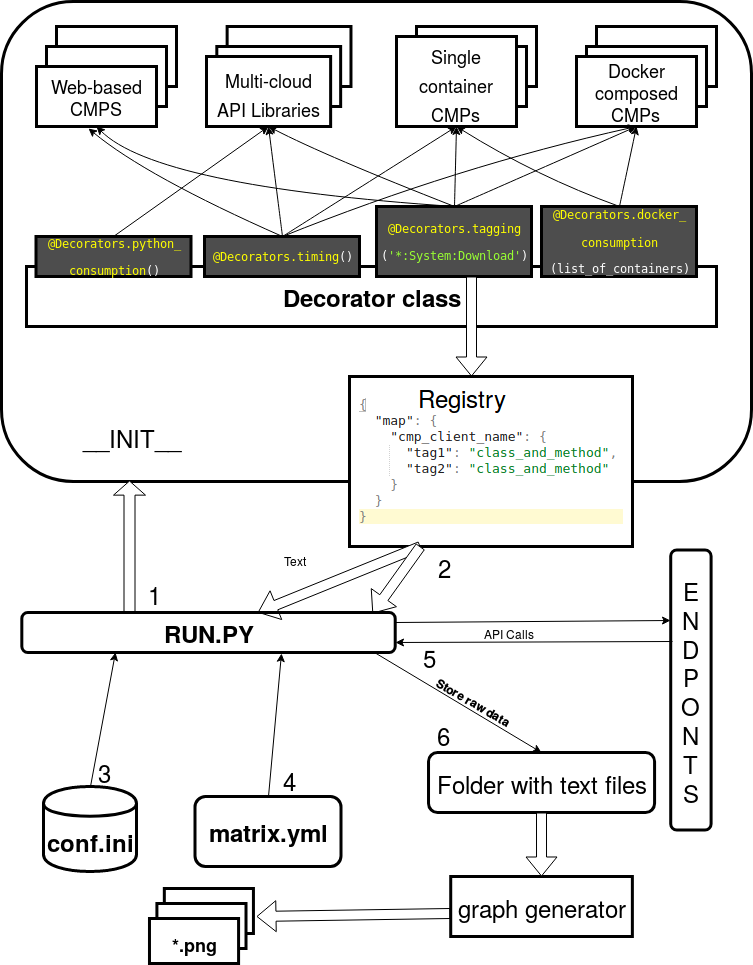
\includegraphics[scale=0.33]{pics/PA1_Diagram.png}}
\caption{Architecture of evaluation application}
\label{fig}
\end{figure}
After reading all the files(configuration and matrix) and creating a common register with the decorator, these data combined and tests produced one by one. Later on, when results are ready, they are dynamically stored in the above folder. In the last step, from the data obtained during the experiment, graphs and matrixes are generated that compare the individual functions.

As it seen the architecture is very flexible and it's easy to add some new platform as well as a characteristic for comparison. With the matrix, it is also possible to create any experiment with the most unusual conditions and the order to evaluate functions and actions
\section{Experiments and results}
\subsection{Experimental setup}
All experiments  launched  on the new virtual machine which is running on OpenStack\cite{openstack} Platform with following characteristics: 
\begin{table}[ht]
\begin{tabular}{ll}
RAM & 4GB \\
VCPUs & 2 VCPU with 2500 Mhz \\
Disk & 40GB \\
OS &  Ubuntu 16.04.4 LTS\\
\end{tabular}
\end{table}

Tests were conducted with each platform 50 times. As evaluation criterion for demonstrating the test environment, used system tests such as download, start, stop, delete. Since CloudchecR is a web-based platform, it was not tested for these characteristics. Also as a testing function used actions with the provider, in this case, each platform worked with an out-of-order provider on AWS server, with the same region and access keys. All of the platforms tested for creation, listing, deleting provider, also ManageIQ and Cloudcheckr for synchronisation time because of architecture design. The following versions of  platforms used in this experiments:

\begin{table}[ht]
\begin{tabular}{ll}
Mist.io  & Cloud Management Platform version: 2.0 \\
ManageIQ & gaprindashvili-3 \\
CloudcheckR & last update May 21, 2018 \\
Apache Libcloud & version 2.3.0\\
\end{tabular}
\end{table}

For the set of the experiments used one single matrix file, which together with raw and aggregated data, can be found along with the source code for this link(put public link).

\subsection{Results}
Architecture of the testbed was designed in that way that overhead is minimal and can be can be neglected.
All the information which given below, such as graphics and tables in the latex format, were generated by the test platform itself. In this part, there will be no in-depth analysis of the data, since comparing different types of platforms is not relevant. The purpose of this work is to provide an approach to creating a test platform for multi-cloud management platforms.

Table \ref{tab:time} shows the results of time evaluation from which concluded that liblcoud performs the fastest system operations since it is an uncomplicated library and it is much simpler than other platforms. Mistio is a multi-image docker platform and because of this loses ManageIQ in the boot time, but shows better results t in time of start and stop the system.

\begin{table}[ht]
\caption{Time criteria exemplary}
\begin{center}
\begin{tabular}{lllllll}
	\hline
	 \multirow{3}{*}{src} & \multirow{3}{*}{action} & \multirow{3}{*}{platform} & \multicolumn{3}{c}{metrics} \\ 
	& & & \multicolumn{3}{c}{time}\\ 
 	& & & mu & sigma & median\\ 
 	\hline
 \\[-1em] \multirow{12}{*}{\rotatebox[origin=c]{90}{*-system}} & \multirow{3}{*}{download} & manageiq & 1.06e+05 & 1.32e+05 & 8.21e+04\\ \\[-1em] 
 	 & & libcloud & 1717.40 & 120.34 & 1711.85\\ \\[-1em] 
 	 & & mistio & 4.25e+05 & 7.21e+05 & 2.58e+05\\ \\[-1em] 
 	\\[-1em] \cline{2-6} \\[-1em] & \multirow{3}{*}{start} & manageiq & 2.00e+05 & 2455.44 & 1.99e+05\\ \\[-1em] 
 	 & & libcloud & 3430.90 & 218.90 & 3445.10\\ \\[-1em] 
 	 & & mistio & 7.93e+04 & 2927.29 & 7.86e+04\\ \\[-1em] 
 	\\[-1em] \cline{2-6} \\[-1em] & \multirow{3}{*}{stop} & manageiq & 654.38 & 92.43 & 645.32\\ \\[-1em] 
 	 & & libcloud & 1575.64 & 125.65 & 1580.09\\ \\[-1em] 
 	 & & mistio & 1.84e+04 & 483.24 & 1.83e+04\\ \\[-1em] 
 	\\[-1em] \cline{2-6} \\[-1em]  & \multirow{3}{*}{remove} & manageiq & 3670.05 & 185.47 & 3669.37\\ \\[-1em] 
 	 & & libcloud & 1.99 & 1.89 & 1.45\\ \\[-1em] 
 	 & & mistio & 6.28e+04 & 7756.02 & 6.08e+04\\ \\[-1em] 
 	 \\[-1em] \hline
	\multirow{14}{*}{\rotatebox[origin=c]{90}{aws-provider}} & \multirow{4}{*}{create} & cloudcheckr & 2411.50 & 263.09 & 2339.36\\ \\[-1em] 
 	 & & manageiq & 254.98 & 140.68 & 225.29\\ \\[-1em] 
 	 & & libcloud & 781.10 & 109.80 & 732.14\\ \\[-1em] 
 	 & & mistio & 1363.78 & 270.84 & 1339.77\\ \\[-1em] 
 	\\[-1em] \cline{2-6} \\[-1em] & \multirow{4}{*}{list} & cloudcheckr & 993.05 & 126.11 & 953.57\\ \\[-1em] 
 	 & & manageiq & 200.26 & 48.64 & 187.33\\ \\[-1em] 
 	 & & libcloud & 338.55 & 38.84 & 328.69\\ \\[-1em] 
 	 & & mistio & 20.77 & 10.16 & 17.31\\ \\[-1em] 
 	\\[-1em] \cline{2-6} \\[-1em] & \multirow{2}{*}{sync} & cloudcheckr & 4.25e+05 & 6.15e+04 & 4.21e+05\\ \\[-1em] 
 	 & & manageiq & 6.94e+05 & 2.06e+06 & 2.75e+04\\ \\[-1em] 
 	\\[-1em] \cline{2-6} \\[-1em] & \multirow{4}{*}{delete} & cloudcheckr & 1063.39 & 192.29 & 1000.20\\ \\[-1em] 
 	 & & manageiq & 7482.43 & 3131.54 & 7014.02\\ \\[-1em] 
 	 & & libcloud & 0.01 & 0.01 & 0.01\\ \\[-1em] 
 	 & & mistio & 103.77 & 41.60 & 88.88\\ \\[-1em] 
 	\\[-1em] \hline
\end{tabular}
\end{center}
\label{tab:time}
\end{table}

In the results of provider operations, liblcoud was again the fastest, from the graphical interface platforms, good results were also shown by the Mistio, unlike ManageIQ and CloudcheckR, there is no need for synchronisation time. At the same time, the creation of the provider the fastest results shown by the ManagqIQ platform that can be seen in figure \ref{creti}.

\begin{figure}[htbp]
\centerline{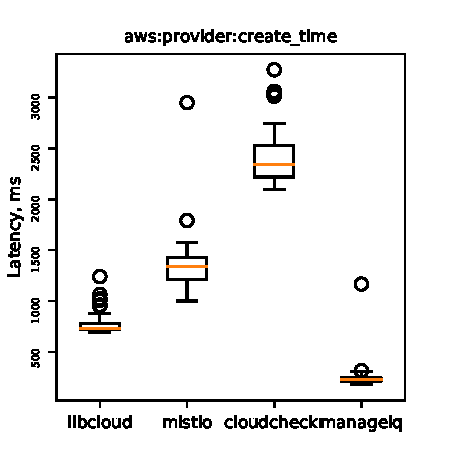
\includegraphics[scale=1]{pics/provider_create_time.pdf}}
\caption{Creation time of provider}
\label{creti}
\end{figure}

Table \ref{tab:cpu} and \ref{tab:mem} show the characteristics of the CPU time and Memory KB
from both results it follows that in docker-base platforms the results are not so stable as seen in figure \ref{crecpu}, but it explained by the fact that the systems are complex and they load themselves, while the operations that were carried out were simple and not resource-intensive, which can be seen from the libcloud on figure \ref{libaws}, were the platform itself is not super resource consumption.
\begin{figure}[htbp]
\centerline{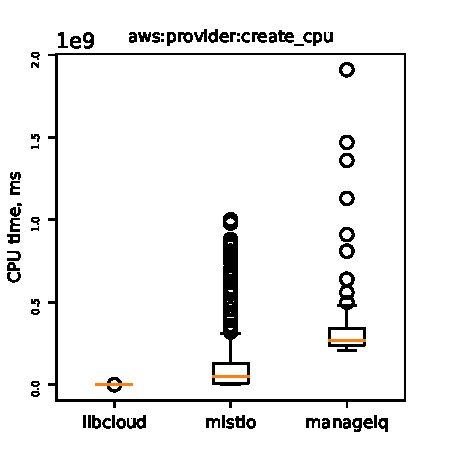
\includegraphics[scale=1]{pics/provider_create_cpu.pdf}}
\caption{Creation CPU time of provider}
\label{crecpu}
\end{figure}

\begin{figure}[htbp]
\centerline{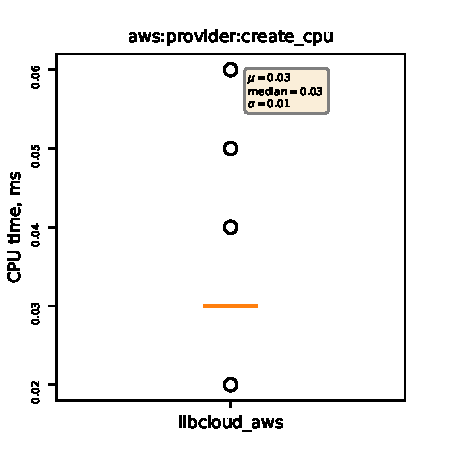
\includegraphics[scale=1]{pics/libcloud_aws.pdf}}
\caption{Creation time of provider}
\label{libaws}
\end{figure}

\begin{table}[ht]
\caption{Creation CPU time of provider for libcloud}
\begin{center}
\begin{tabular}{lllllll}
	\hline
	\multirow{3}{*}{src} & \multirow{3}{*}{action} & \multirow{3}{*}{platform} & \multicolumn{3}{c}{metrics} \\ 
	& & & \multicolumn{3}{c}{cpu}\\ 
 	& & & mu & sigma & median\\ 
 	\hline
 \\[-1em] \multirow{10}{*}{\rotatebox[origin=c]{90}{aws-provider}} & \multirow{3}{*}{create} & manageiq & 4.24e+08 & 3.67e+08 & 2.70e+08\\ \\[-1em] 
 	 & & libcloud & 0.03 & 0.01 & 0.03\\ \\[-1em] 
 	 & & mistio & 1.12e+08 & 1.74e+08 & 5.00e+07\\ \\[-1em] 
 	\\[-1em] \cline{2-6} \\[-1em] & \multirow{3}{*}{list} & manageiq & 5.88e+08 & 3.60e+08 & 4.40e+08\\ \\[-1em] 
 	 & & libcloud & 0.01 & 0.01 & 0.01\\ \\[-1em] 
 	 & & mistio & 9.34e+07 & 1.79e+08 & 3.00e+07\\ \\[-1em] 
 	\\[-1em] \cline{2-6} \\[-1em]  & \multirow{1}{*}{sync} & manageiq & 6.58e+11 & 1.93e+12 & 3.37e+10\\ \\[-1em] 
 	\\[-1em] \cline{2-6} \\[-1em]  & \multirow{3}{*}{delete} & manageiq & 7.62e+09 & 5.42e+09 & 6.36e+09\\ \\[-1em] 
 	 & & libcloud & 0.00 & 0.00 & 0.00\\ \\[-1em] 
 	 & & mistio & 9.30e+07 & 1.52e+08 & 4.00e+07\\ \\[-1em] 
 	\\[-1em] \hline
\end{tabular}
\end{center}
\label{tab:cpu}
\end{table}

\begin{table}[ht]
\caption{Memory KB criteria evaluation}
\begin{center}
\begin{tabular}{lllllll}
	\hline
	\multirow{3}{*}{src} & \multirow{3}{*}{action} & \multirow{3}{*}{platform} & \multicolumn{3}{c}{metrics} \\ 
	& & & \multicolumn{3}{c}{memory}\\ 
 	& & & mu & sigma & median\\ 
 	\hline
 \\[-1em] \multirow{10}{*}{\rotatebox[origin=c]{90}{aws-provider}} & \multirow{3}{*}{create} & manageiq & -1.40e+07 & 7.38e+07 & 7.37e+04\\ \\[-1em] 
 	 & & libcloud & 2.73e+05 & 4.31e+05 & 0.00\\ \\[-1em] 
 	 & & mistio & 4.04e+05 & 5.46e+06 & 0.00\\ \\[-1em] 
 	\\[-1em] \cline{2-6} \\[-1em] & \multirow{3}{*}{list} & manageiq & 2.82e+06 & 1.56e+07 & 1.68e+05\\ \\[-1em] 
 	 & & libcloud & 1.11e+04 & 4.64e+04 & 0.00\\ \\[-1em] 
 	 & & mistio & 3.08e+04 & 6.05e+06 & 0.00\\ \\[-1em] 
 	\\[-1em] \cline{2-6} \\[-1em] & \multirow{1}{*}{sync} & manageiq & 2.00e+08 & 9.66e+07 & 1.75e+08\\ \\[-1em] 
 	\\[-1em] \cline{2-6} \\[-1em] & \multirow{3}{*}{delete} & manageiq & -1.63e+08 & 7.67e+07 & -1.76e+08\\ \\[-1em] 
 	 & & libcloud & 0.00 & 0.00 & 0.00\\ \\[-1em] 
 	 & & mistio & -1.47e+05 & 6.56e+06 & 0.00\\ \\[-1em] 
 	\\[-1em] \hline
\end{tabular}
\end{center}
\label{tab:mem}
\end{table}


\section{Conclusion}
With the popularity of hybrid cloud systems, the number of platforms trying to centralise their management and the billing system is continuously growing. This Cloud management platform differs depending on the software, and each of them is suitable for specific purposes. A lot of works that compare a separate platform functionality are written and published, which indicates the relevance of this topic. In this paper, we examined the possibility of centralised and standardised testing of CMPs based on web platforms, local docker platforms and libraries.

As part of this work written a test environment and created an architecture for multi-platform testing that systematised comparisons and provides the ability to run all tests with just one starting file, which in the future can be used by other researchers to validate the experiments. The architecture is modular and very flexible, which provides the possibility of its constant expansion. The raw result stored in text form, which in the future by the same test-bed generates not only single and combined graphs, but also tables in latex format.

The aim of the work was not to compare the platforms but to create a test environment and, as an example used libcloud (library), mistio(docker composed containers), ManageIQ(single image container), CloudcheckR(website with open API). The results are entirely consistent since libraries are the easiest way to manage platforms and they do not have an overhead, and they showed the best results. In the evaluation of provider management between two local running platforms mistio showed itself better since ManageIQ has the much more full range of functionality and possibilities leading to more significant overhead.
All the data and findings published in opensource to keep the studying reusable and repeatable.
\bibliography{references}
\bibliographystyle{unsrt}



\endgroup
\end{document}